
% LaTeX Language and campus name and format package
\documentclass[es,gi]{ifirak}\usepackage[]{graphicx}\usepackage[]{color}
%% maxwidth is the original width if it is less than linewidth
%% otherwise use linewidth (to make sure the graphics do not exceed the margin)
\makeatletter
\def\maxwidth{ %
  \ifdim\Gin@nat@width>\linewidth
    \linewidth
  \else
    \Gin@nat@width
  \fi
}
\makeatother

\definecolor{fgcolor}{rgb}{0.345, 0.345, 0.345}
\newcommand{\hlnum}[1]{\textcolor[rgb]{0.686,0.059,0.569}{#1}}%
\newcommand{\hlstr}[1]{\textcolor[rgb]{0.192,0.494,0.8}{#1}}%
\newcommand{\hlcom}[1]{\textcolor[rgb]{0.678,0.584,0.686}{\textit{#1}}}%
\newcommand{\hlopt}[1]{\textcolor[rgb]{0,0,0}{#1}}%
\newcommand{\hlstd}[1]{\textcolor[rgb]{0.345,0.345,0.345}{#1}}%
\newcommand{\hlkwa}[1]{\textcolor[rgb]{0.161,0.373,0.58}{\textbf{#1}}}%
\newcommand{\hlkwb}[1]{\textcolor[rgb]{0.69,0.353,0.396}{#1}}%
\newcommand{\hlkwc}[1]{\textcolor[rgb]{0.333,0.667,0.333}{#1}}%
\newcommand{\hlkwd}[1]{\textcolor[rgb]{0.737,0.353,0.396}{\textbf{#1}}}%
\let\hlipl\hlkwb

\usepackage{framed}
\makeatletter
\newenvironment{kframe}{%
 \def\at@end@of@kframe{}%
 \ifinner\ifhmode%
  \def\at@end@of@kframe{\end{minipage}}%
  \begin{minipage}{\columnwidth}%
 \fi\fi%
 \def\FrameCommand##1{\hskip\@totalleftmargin \hskip-\fboxsep
 \colorbox{shadecolor}{##1}\hskip-\fboxsep
     % There is no \\@totalrightmargin, so:
     \hskip-\linewidth \hskip-\@totalleftmargin \hskip\columnwidth}%
 \MakeFramed {\advance\hsize-\width
   \@totalleftmargin\z@ \linewidth\hsize
   \@setminipage}}%
 {\par\unskip\endMakeFramed%
 \at@end@of@kframe}
\makeatother

\definecolor{shadecolor}{rgb}{.97, .97, .97}
\definecolor{messagecolor}{rgb}{0, 0, 0}
\definecolor{warningcolor}{rgb}{1, 0, 1}
\definecolor{errorcolor}{rgb}{1, 0, 0}
\newenvironment{knitrout}{}{} % an empty environment to be redefined in TeX

\usepackage{alltt}

% ERABILIKO DIREN PAKETEAK %

% listings pakage is for code formating
\usepackage{listings}
% Paquete for acents and other special characters
% It is not necesary to use all this packages add or remove those you are interested on
\usepackage[utf8]{inputenc}
\usepackage{colortbl}
\usepackage[table]{xcolor}
\usepackage{graphicx}
\usepackage{wrapfig}
\usepackage{amsfonts}
\usepackage{makeidx}
\usepackage{adjustbox}
\usepackage{booktabs}
\usepackage{amsmath}

% Definition of colors
\definecolor{darkgreen}{rgb}{0,0.5,0}
\definecolor{lightgray}{rgb}{0.95,0.95,0.95}
\definecolor{gray}{rgb}{0.85,0.85,0.85}
\definecolor{white}{rgb}{1,1,1}
\definecolor{purple}{rgb}{0.51,0,0.25}
\definecolor{orange}{rgb}{0.255,0.178,0.102}
\definecolor{mygreen}{RGB}{28,172,0} 
\definecolor{mylilas}{RGB}{170,55,241}

\lstset{language=Matlab,%
    %basicstyle=\color{red},
    breaklines=true,%
    morekeywords={matlab2tikz},
    keywordstyle=\color{blue},%
    morekeywords=[2]{1}, keywordstyle=[2]{\color{black}},
    identifierstyle=\color{black},%
    stringstyle=\color{mylilas},
    commentstyle=\color{mygreen},%
    showstringspaces=false,%without this there will be a symbol in the places where there is a space
    %numbers=left,%
    %numberstyle={\tiny \color{black}},% size of the numbers
    %numbersep=20pt, % this defines how far the numbers are from the text
    emph=[1]{for,end,break},emphstyle=[1]\color{red}, %some words to emphasise
    %emph=[2]{word1,word2}, emphstyle=[2]{style},    
    backgroundcolor=\color{lightgray},
}

\DeclareMathSizes{10}{10}{10}{10}

\graphicspath{imagenes}
\renewcommand{\contentsname}{Indice}
\IfFileExists{upquote.sty}{\usepackage{upquote}}{}
\begin{document}

% Course year
\ikasturtea{2018 - 2019}
% Subject or course name
\irakasgaia{Visión por Computador}
% Title
\title{Desafíos 5, 6 y 7}
% Name of Author
\author{Mikel Dalmau}

\maketitle



%\section{Código}

\tableofcontents

\pagebreak
\section{Enunciados}
\subsection{Desafío 5}
\paragraph{} El objetivo del desafío es construir un clasificador basado en las signaturas de color de las imágenes para ello será necesario crear un mapa de colores de los objetos y clasificar las imágenes en función de los histogramas de color utilizando la herramienta Matlab \textit{rgb2ind}.\\

Para el desafío se utilizarán las imagenes en la base de datos COIL-100 \cite{key-2}.

\subsection{Desafío 6}
\paragraph{}El objetivo de este desafío es construir un clasificador basado en las características construidas por el método del histograma de gradiente, en Matlab \textit{extractHOGFeatures}.\\

La idea general es construir un clasificador 1-NN con las características extraídas de los representantes de los objectos usados como conjunto de entrenamiento, usar una celda relativamente grande (32x32) para obtener vectores de características de un tamaño no excesivo.\\

Estudiar cuantas vistas/ángulos son necesarios para obtener resultados "aceptables" y cual es el balance entre tamaños de conjuntos de entrenamiento y test.\\

\subsection{Desafío 7}
\paragraph{}El objetivo de este desafío es realizar la clasificación de los objetos utilizando las funciones de emparejamiento de características de imágenes disponibles en el computer vision toolbox de Matlab. El proceso primeramente detecta puntos característicos, después extrae información discriminante en la región entorno al punto característico y usa esa información para calcular emparejamientos de puntos característicos entre imágenes.\\

Herramienta Matlab : \textit{detectSURFFeatures}, \textit{extractFeatures}, \textit{matchFeatures}\\


La idea general es considerar las imágenes de entrenamiento como una escena  de referencia donde queremos localizar el objecto a clasificar, la identificación de la clase corresponde a la sub-imagen en la que obtenemos más correspondencias.

\pagebreak
\section{El conjunto de datos}

\paragraph{} La base de imágenes COIL-100 está compuesta por imágenes de 100 objectos distintos, colocados sobre un fondo negro. De cada objecto se han creado 72 imágenes y corresponden a las rotaciones de $5^{\circ}$ de cada imagen desde $0^{\circ}$ hasta $355^{\circ}$. Las imágenes tienen todas las mismas dimensiones 128x128x3.\\

De acuerdo a estas características, la nomenclatura de las imágenes sigue el formato:  \textit{obj$\lbrace$numero imagen$\rbrace$\\ \_\_$\lbrace$angulo$\rbrace$.png}. Véanse un par de ejemplos de imágenes presentes en COIL-100.\\

\vspace*{1cm}

\begin{tabular}{ccccc}
    \toprule
    
	\bfseries Nombre &
    \bfseries $0^{\circ}$ &
    \bfseries $90^{\circ}$ &
   	\bfseries $180^{\circ}$&
   	\bfseries $270^{\circ}$\\
    
    \midrule
    	obj1
		& \adjustimage{height=3cm,valign=m}{imagenes/obj1__0}
		
		& \adjustimage{height=3cm,valign=m}{imagenes/obj1__90}	
		& \adjustimage{height=3cm,valign=m}{imagenes/obj1__180}
		& \adjustimage{height=3cm,valign=m}{imagenes/obj1__270}\\
		\\
		obj53
		& \adjustimage{height=3cm,valign=m}{imagenes/obj53__0}
		& \adjustimage{height=3cm,valign=m}{imagenes/obj53__90}	
		& \adjustimage{height=3cm,valign=m}{imagenes/obj53__180}
		& \adjustimage{height=3cm,valign=m}{imagenes/obj53__270}\\
		\\
		obj100
		& \adjustimage{height=3cm,valign=m}{imagenes/obj100__0}
		& \adjustimage{height=3cm,valign=m}{imagenes/obj100__90}	
		& \adjustimage{height=3cm,valign=m}{imagenes/obj100__180}
		& \adjustimage{height=3cm,valign=m}{imagenes/obj100__270}\\
		
	\midrule
    \bottomrule
\end{tabular}

\vspace*{1cm}
\paragraph{*}La figura 7 muestra stodos los objetos de COIL-100 para el ángulo 0.
\pagebreak
\section{Desafío 5: Clasificar por colores}
\subsection{Extracción del mapa de colores}
\paragraph{} El primer paso para crear el clasificador es indexar las imágenes de forma que cada pixel de la imagen será sustituido por un índice al mapa de colores. De cara a indexar todas las imágenes es conveniente que todas utilicen el mismo mapa de colores, para ello la estrategia utilizada consiste en unir una imagen de cada clase e indexar la unión.\\

Para el indexado se utiliza la función de \textit{rgb2ind}, y como parámetros la imagen conjunta y el número de colores para indexar, en este caso 256 y da como resultado la imagen indexada y su mapa, el siguiente código realiza dichas operaciones.\\

\begin{figure}[hbtp]
\centering
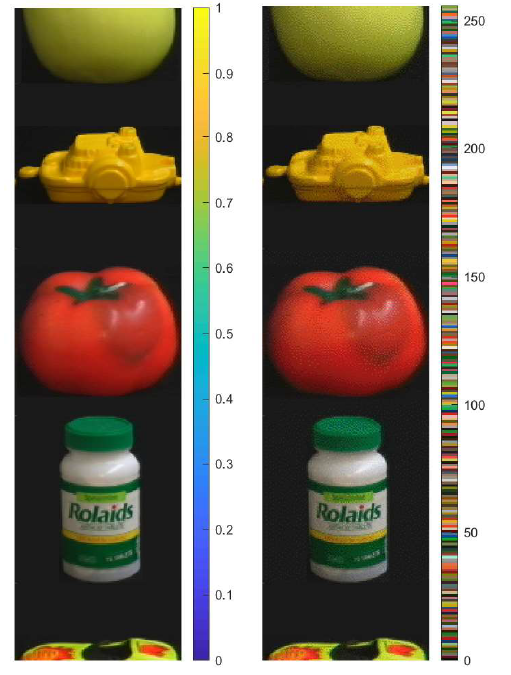
\includegraphics[scale=0.75]{imagenes/ConjutaEIndexada.png}
\caption{Sección de la imagen conjunta a la izquierda y la indexada a la derecha. Las barras de colores laterales muestran el mapa de colores de cada una, puede distinguirse como la imagen indexada ha perdido algunos de sus colores y estos se han sustituido por los más similares pertenecientes al mapa.}
\end{figure}

\begin{lstlisting}
%% Construir la muestra de colores
% clases -> Numero de clases
% theta -> Angulo del representante
% h -> Altura de las imagenes
% w -> anchura de las imagenes
% colores -> Numero de colores del indexado
function mct = calcularMapaDeColores(clases,theta,h,w,colores)

    % Inicializamos la matriz que contendra todas las imagenes de muestra y de
    % la que extraeremos el mapa de colores con el que trabajar.
    %
    %  *Concatenaremos las imagenes en la primera dimension, por lo que los valores
    %   para la 2nda y la 3a dimension se mantienen iguales.
    %
    muestra=uint8(zeros(h*clases,w,3));

    % Leemos las imagenes que tienen angulo Theta y creamos el mapa de colores
    % con ellas
    for i = 1:clases

        % Rellenamos la muestra
        imageName = "obj"+i+"__"+theta+".png";
        muestra((i-1)*h+1:i*h,1:w,1:3) = imread(imageName);
    end
    
    % Extraccion del mapa de colores y muestra indexada a partir de la muestra
    [~,mct] = rgb2ind(muestra,colores);     
end
\end{lstlisting}

\subsection{Creación de los representantes o conjunto de entrenamiento}
\paragraph{} El siguiente paso, una vez calculado el mapa, consiste en elegir los representantes, indexarlos $\left( usando\ rgb2ind \right)$ utilizando el mapa y crear un histograma a partir de los índices usando la función de matlab \textit{imhist}, esta función nos devuelve un vector de igual longitud al mapa de colores donde la posición del vector representa un color y el número en dicha posición las veces que ese color ha sido indexado.\\

Finalmente guardo para cada representante calculado, su clase o lo que es lo mismo el número de objeto que tiene, y su histograma.\\

El siguiente código realiza este paso y permite pasándole un vector de ángulos especificar que ángulos de imágenes se usarán para calcular los representantes.

\begin{lstlisting}
% El resultado es una matriz de celdas con los histogramas representantes de cada clase
function reps = calcularRepresentantes(clases,angulos, mct)
    reps = cell(clases*length(angulos),2);
    k = 1;
    % Para cada clase
    for i=1:clases
        % Para cada angulo en angulos de cada clase
        for j = 1:length(angulos)
            imageName = "obj"+i+"__"+angulos(j)+".png";
            [contadores,~]=imhist(rgb2ind(imread(imageName),mct),mct);
            reps(k,1:2)={i,contadores};
            k=k+1;
        end 
    end
end
\end{lstlisting}

\subsection{Algoritmo de clasificación}
\paragraph{} Una vez definido el método de indexado y definidos los representantes como histogramas de colores. El siguiente paso es indexar el resto de imágenes, extraer sus histogramas y clasificarlas. En este caso se ha utilizado el algoritmo 1-NN (1 - Nearest Neighbour) y como métrica de comparación se ha utilizado la norma euclídea, esto es, se asignará a una imagen la clase de aquel representante cuya norma vectorial entre sus histogramas sea la mínima.

\begin{lstlisting}
%% Clasificacion de las imagenes
function clasificacion = clasificar(clases,reps,angulos,mct)

    % Matriz de pares con el numero de clase real y clasificado
    clasificacion = zeros(clases*(72 - length(angulos)),1);
    
    % Para cada clase de 1 a 100
    j = 1;
    for i = 1:clases
        % Para cada angulo de 0 a 355 (de 5 en 5 grados)
        for theta = 0:5:355
            if ~ismember(theta,angulos)
                imageName = "obj"+i+"__"+theta+".png";

                % Indexar y sacar el histograma
                indexada = rgb2ind(imread(imageName),mct);
                [contadores,~]=imhist(indexada,mct);

                % Clasificar
                clase = NN_1(reps,contadores);

                clasificacion(j,1:2) = [i, clase];
                j = j+1;
            end
        end 
    end
end

% NN_1 
function clase = NN_1(reps, aClasificar)
    
    min = intmax();
    clase = 0;
    
    for i = 1:length(reps)
        clase_temp = reps{i,1};
        hist = reps{i,2};
        norma = norm(hist-aClasificar);
        
        if norma < min 
            clase = clase_temp;
            min = norma;
        end 
    end
end

\end{lstlisting}

\subsection{Resultados}
\paragraph{} En esta sección exploramos los resultados de aplicar el proceso anterior con distintos parámetros, variando el número de representantes y sus ángulos.\\

También intentaremos ver la clasificación de que objetos mejora al aumentar los representantes y para que objetos no es tan relevante la mejora y que características de los objetos explican este problema.\\

\begin{tabular}{ccccc}
 \toprule
	\bfseries Prueba &
    \bfseries Representantes &
	\bfseries Angulos de Rep.&
	\bfseries Tamaño del conjunto de test &
	\bfseries \% acierto \\
 \midrule
	1 & 100 (1.4\%) & 0 & 7100 (98.6\%) & 59.2 \\
	2 & 400 (5.5\%)& 0, 90, 180, 270 & 6800 (94.5\%) & 78.09\\
	3 & 800 (11.1\%)& 0, 45, 90, 135, 180, 225, 270, 315 & 6400 (88.9\%) & 89.86\\
 \bottomrule
\end{tabular}

\vspace{0.3cm}

En la siguiente tabla se muestran algunos de los objetos mejor clasificados en el primer test ( con 1 solo representante por clase) y los objetos peor clasificados en el test 3 (8 represnetantes por clase).\\

La conclusión que extraemos de estos resultados es que la geometría del objeto es el principal factor a la hora de determinar el éxito en la clasificación junto con las similitudes en el color. De esta forma, los objetos que tienen geometrías regulares respecto a su eje vertical y no cambian al ser rotadas, como las que vemos en el ejemplo: un toro, una sección de cono y 2 cilindros se clasifican con mucho más éxito que las otras.\\

\begin{tabular}{ccc|ccc}
 \toprule
	\bfseries Objeto &
    \bfseries \% Aciertos (p1) &
	\bfseries Imagen &
	
	\bfseries Objeto &
	\bfseries \% Aciertos (p3)&
	\bfseries Imagen\\
 \midrule
	95 & 100 & \adjustimage{height=2.8cm,valign=m}{imagenes/obj95__0} & 65 & 37.5 & \adjustimage{height=2.8cm,valign=m}{imagenes/obj65__0}\\
	\\
	94 & 100 & \adjustimage{height=2.8cm,valign=m}{imagenes/obj94__0} & 68 & 39 & \adjustimage{height=2.8cm,valign=m}{imagenes/obj68__0}  \\
	\\
	93 & 100 & \adjustimage{height=2.8cm,valign=m}{imagenes/obj93__0} & 51 & 48.4 & \adjustimage{height=2.8cm,valign=m}{imagenes/obj51__0}\\
	\\
	87 & 100 & \adjustimage{height=2.8cm,valign=m}{imagenes/obj87__0} & 80 & 51.5 & \adjustimage{height=2.8cm,valign=m}{imagenes/obj80__0} \\
 \midrule
 \bottomrule
\end{tabular}

\begin{figure}[hbtp]
\centering
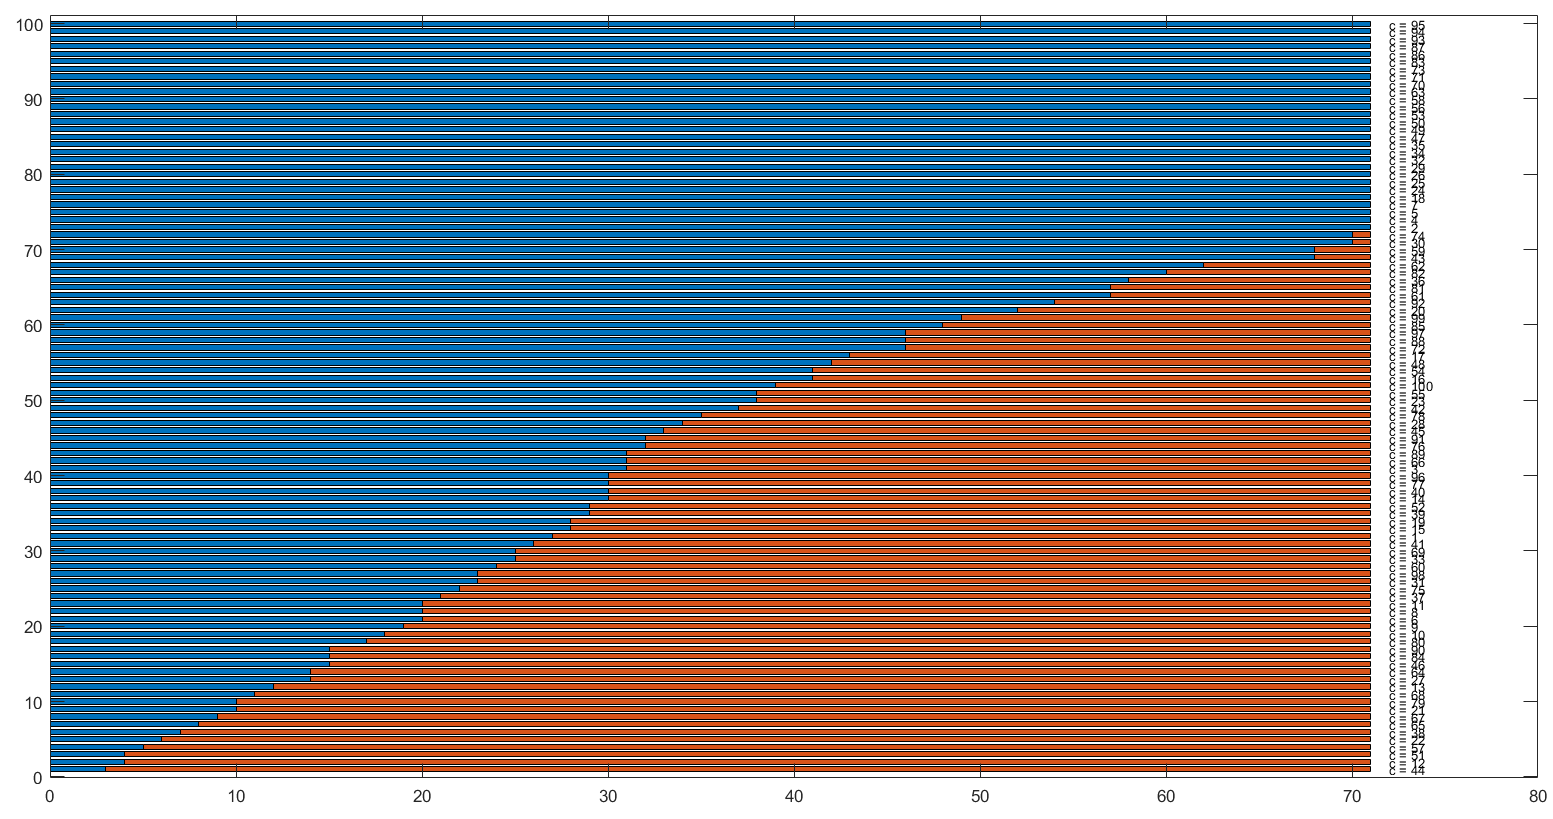
\includegraphics[scale=0.35]{imagenes/histo1.png}
\caption{Ranking de exitos por clase para la prueba 1.}
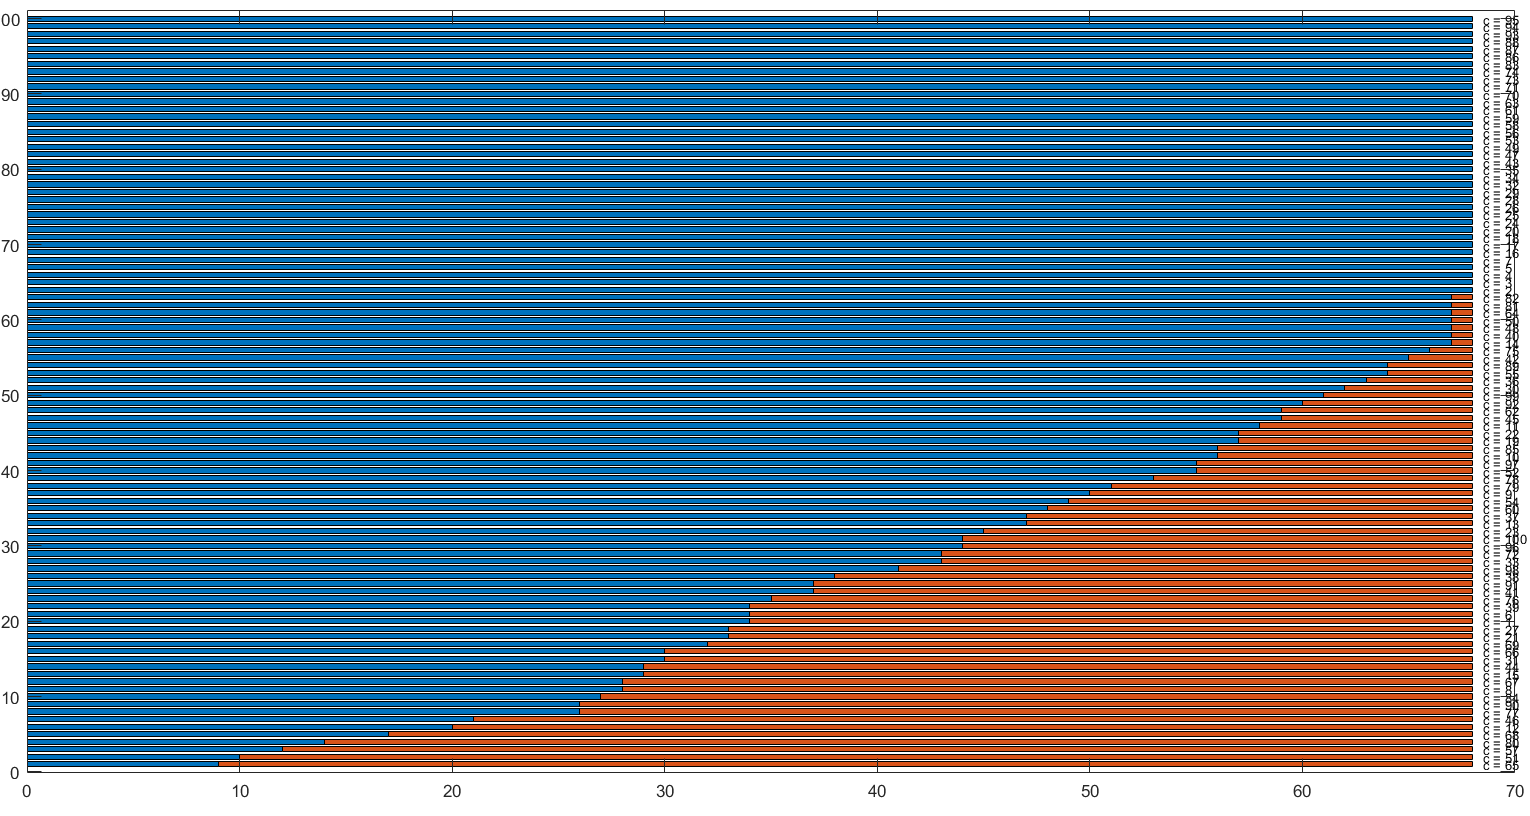
\includegraphics[scale=0.35]{imagenes/histo2.png}
\caption{Ranking de exitos por clase para la prueba 2.}
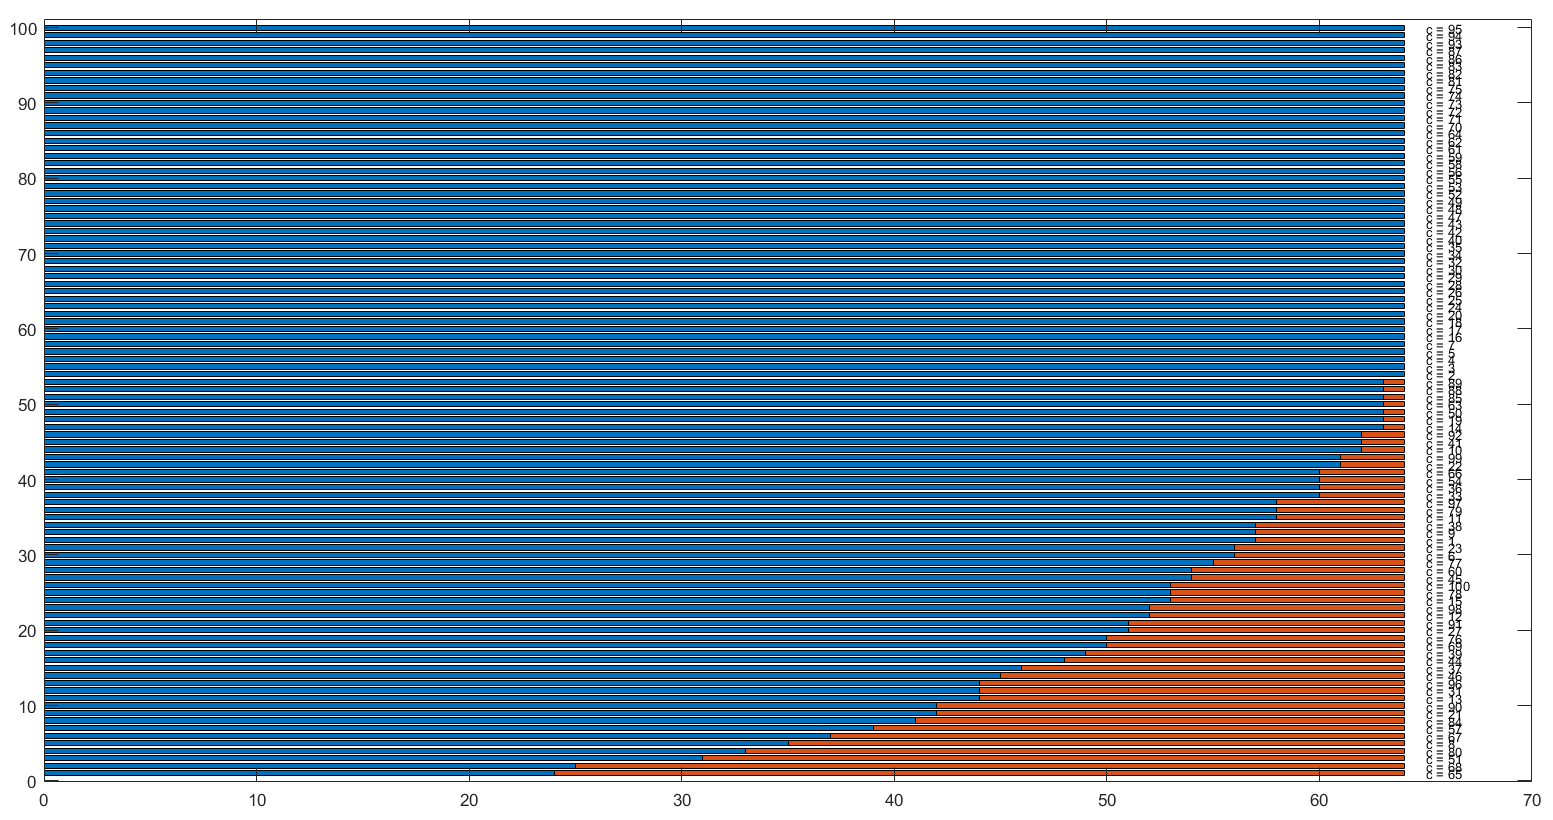
\includegraphics[scale=0.35]{imagenes/histo3.png}
\caption{Ranking de exitos por clase para la prueba 3.}
\end{figure}

\pagebreak

\section{Desafío 6: Clasificar por gradientes}
\paragraph{} El método de clasificar por gradientes consiste en primer lugar en extraer información sobre la orientación de la imagen en distintos puntos de esta. Para esto se divide la imagen y utilizan matrices de convolución que calculan los gradientes o bordes de las sub imagenes, luego se redondean las direcciones de los bordes a unas direcciones privilegiadas y se crea un histograma con estas. Finalmente uniendo todos los histogramas de las sub-imagenes se obtiene un histograma global que podemos utilizar para comparar con otros utilizando alguna métrica como la norma euclídea.\\


\begin{figure}[hbtp]
\centering
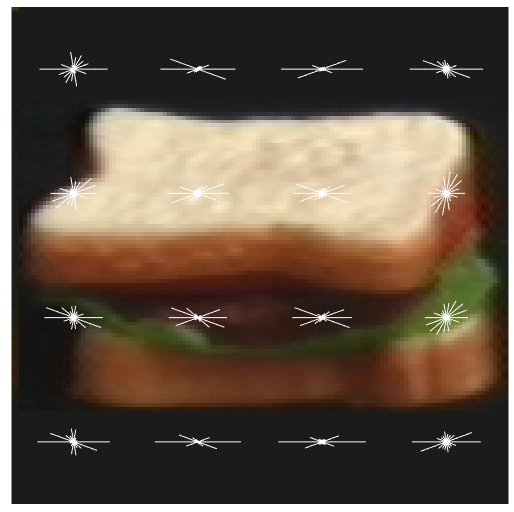
\includegraphics[scale=0.6]{imagenes/sandw.png}
\caption{Figura con sus histogramas de orientaciones representados de forma polar.}
\end{figure}

\pagebreak
\subsection{El algoritmo de clasificación}
\paragraph{} De cara a encontrar una buena relación entre el número de imágenes de test y un resultado aceptable he modificado el código a disposición en clase para que compare los histogramas de gradientes de varias imágenes en vez de hacerlo con solo una imagen.\\

Intuitivamente y como ya hemos visto en otros desafíos sobre COIL-100, conviene que los representantes no tengan ángulos similares para mejorar la clasificación ya que así es más probable que el caso a clasificar se encuentre próximo a uno de ellos. Por esto, he modificado el código para que cree conjuntos de representantes equi-espaciados y he hecho pruebas para conjuntos de tamaño $1 \leftarrow ([1],[2],[3]...[72])$ de tamaño $4 \leftarrow ([1,19,37,56]...[18,36,54,72])$ y de tamaño 8.\\

\begin{lstlisting}
%% Leer los datos
caracteristicas = cell(100,72);
for obj=1:100
    for vista = 1:72
        imageName = "obj"+obj+"__"+(5*(vista-1))+".png";
        caracteristicas{obj,vista}=extractHOGFeatures(imread(imageName),'CellSize',[32, 32]);
    end
end

confusion=zeros(100);
vistasTestSize = 1;
shift = 72/vistasTestSize;
for i=1:shift
    vistas_train = i:shift:i+(vistasTestSize-1)*shift;
    for vista_test=1:72
        if ~ismember(vista_test,vistas_train)
            for obj_test=1:100
                dist=[100*length(vistas_train) 2];
                
                k = 1;
                for obj_train=1:100
                    for j = 1:length(vistas_train)
                        dist(k,:)=[obj_train, norm(caracteristicas{obj_train,vistas_train(j)}-caracteristicas{obj_test,vista_test})];
                        k = k + 1;
                    end
                end

                [m,obj_m]=min(dist(:,2));
                obj_min = dist(obj_m,1);
                confusion(obj_test,obj_min)=confusion(obj_test,obj_min)+1;
            end
        end
    end
end
\end{lstlisting}

\pagebreak
\subsection{Resultados}
\paragraph{} 

En la siguiente tabla se muestran algunos de los objetos mejor clasificados en el primer test ( con 1 solo representante por clase) y los objetos peor clasificados en el test 3 (8 representantes por clase).\\

\begin{tabular}{ccccc}
 \toprule
	\bfseries Prueba &
    \bfseries Representantes &
	\bfseries Tamaño del conjunto de test &
	\bfseries \% acierto  &
	\bfseries Desv. Std.\\
 \midrule
	1 & 100 (1.4\%) & 7100 (98.6\%) & 48.71 & 0.3236 \\
	2 & 400 (5.5\%) & 6800 (94.5\%) & 73.42 &  0.2548\\
	3 & 800 (11.1\%) & 6400 (88.9\%) & 89.80 & 0.1434\\
 \bottomrule
\end{tabular}

\paragraph{}
La conclusión que extraemos de estos resultados es otra vez que la geometría del objeto es el principal factor favoreciendo a los objetos que tienen geometrías regulares respecto a su eje vertical y no cambian al ser rotadas frente a los objetos rectangulares que son los que peor se clasifican, a diferencia de la clasificación anterior, estos objetos no habían quedado últimos debido a sus colores homogéneos.\\

\begin{tabular}{ccc|ccc}
 \toprule
	\bfseries Objeto &
    \bfseries \% Aciertos (p1) &
	\bfseries Imagen &
	\bfseries Objeto &
	\bfseries \% Aciertos (p3)&
	\bfseries Imagen\\
 \midrule
	95 & 100 & \adjustimage{height=2.8cm,valign=m}{imagenes/obj95__0} & 98 & 41 & \adjustimage{height=2.8cm,valign=m}{imagenes/obj98__0}\\
	\\
	94 & 100 & \adjustimage{height=2.8cm,valign=m}{imagenes/obj94__0} & 96 & 46.4 & \adjustimage{height=2.8cm,valign=m}{imagenes/obj96__0}  \\
	\\
	86 & 100 & \adjustimage{height=2.8cm,valign=m}{imagenes/obj86__0} & 84 & 55.3 & \adjustimage{height=2.8cm,valign=m}{imagenes/obj84__0}\\
	\\
	58 & 100 & \adjustimage{height=2.8cm,valign=m}{imagenes/obj58__0} & 67 & 55.4 & \adjustimage{height=2.8cm,valign=m}{imagenes/obj67__0} \\
 \midrule
 \bottomrule
\end{tabular}

\begin{figure}[hbtp]
\centering
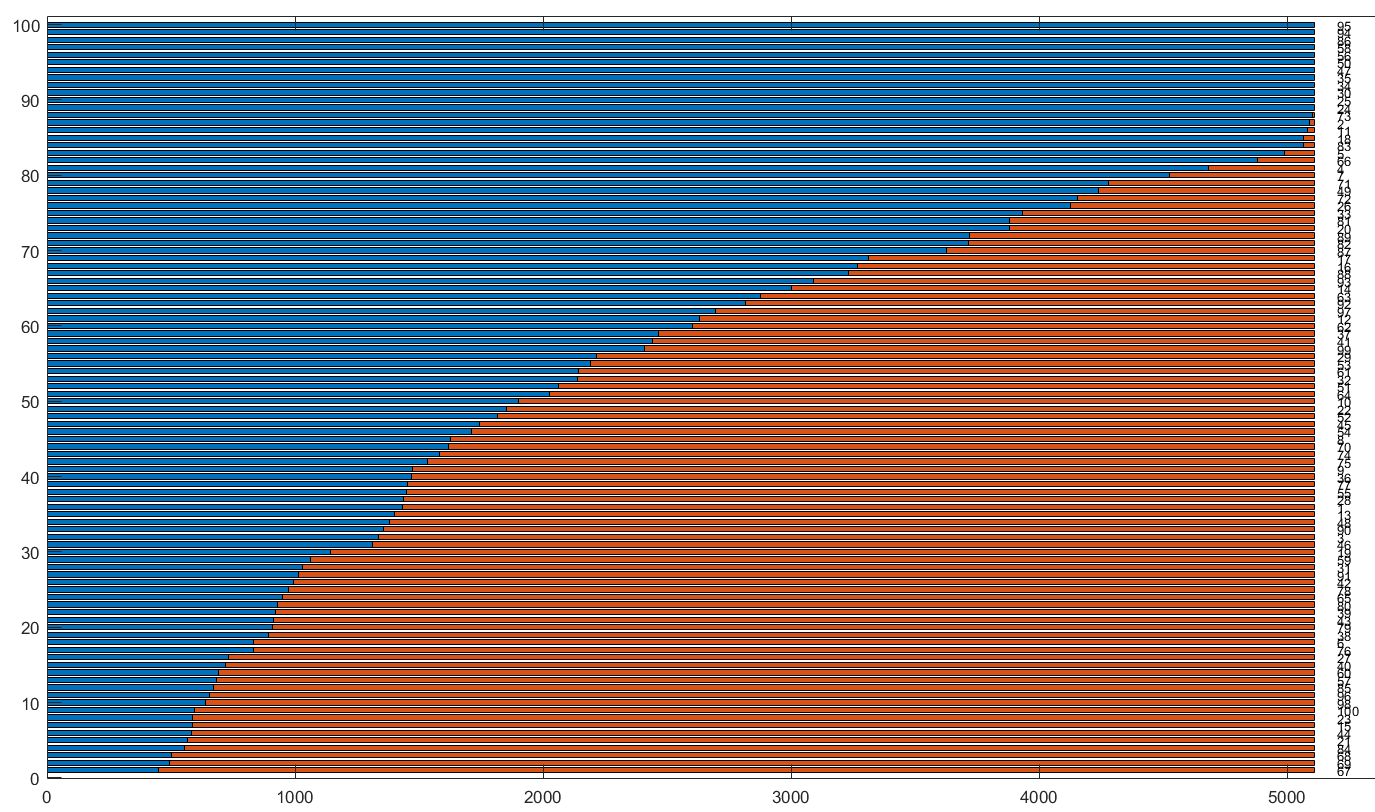
\includegraphics[scale=0.35]{imagenes/histo1_desafio6.png}
\caption{Ranking de exitos por clase para la prueba 1.}
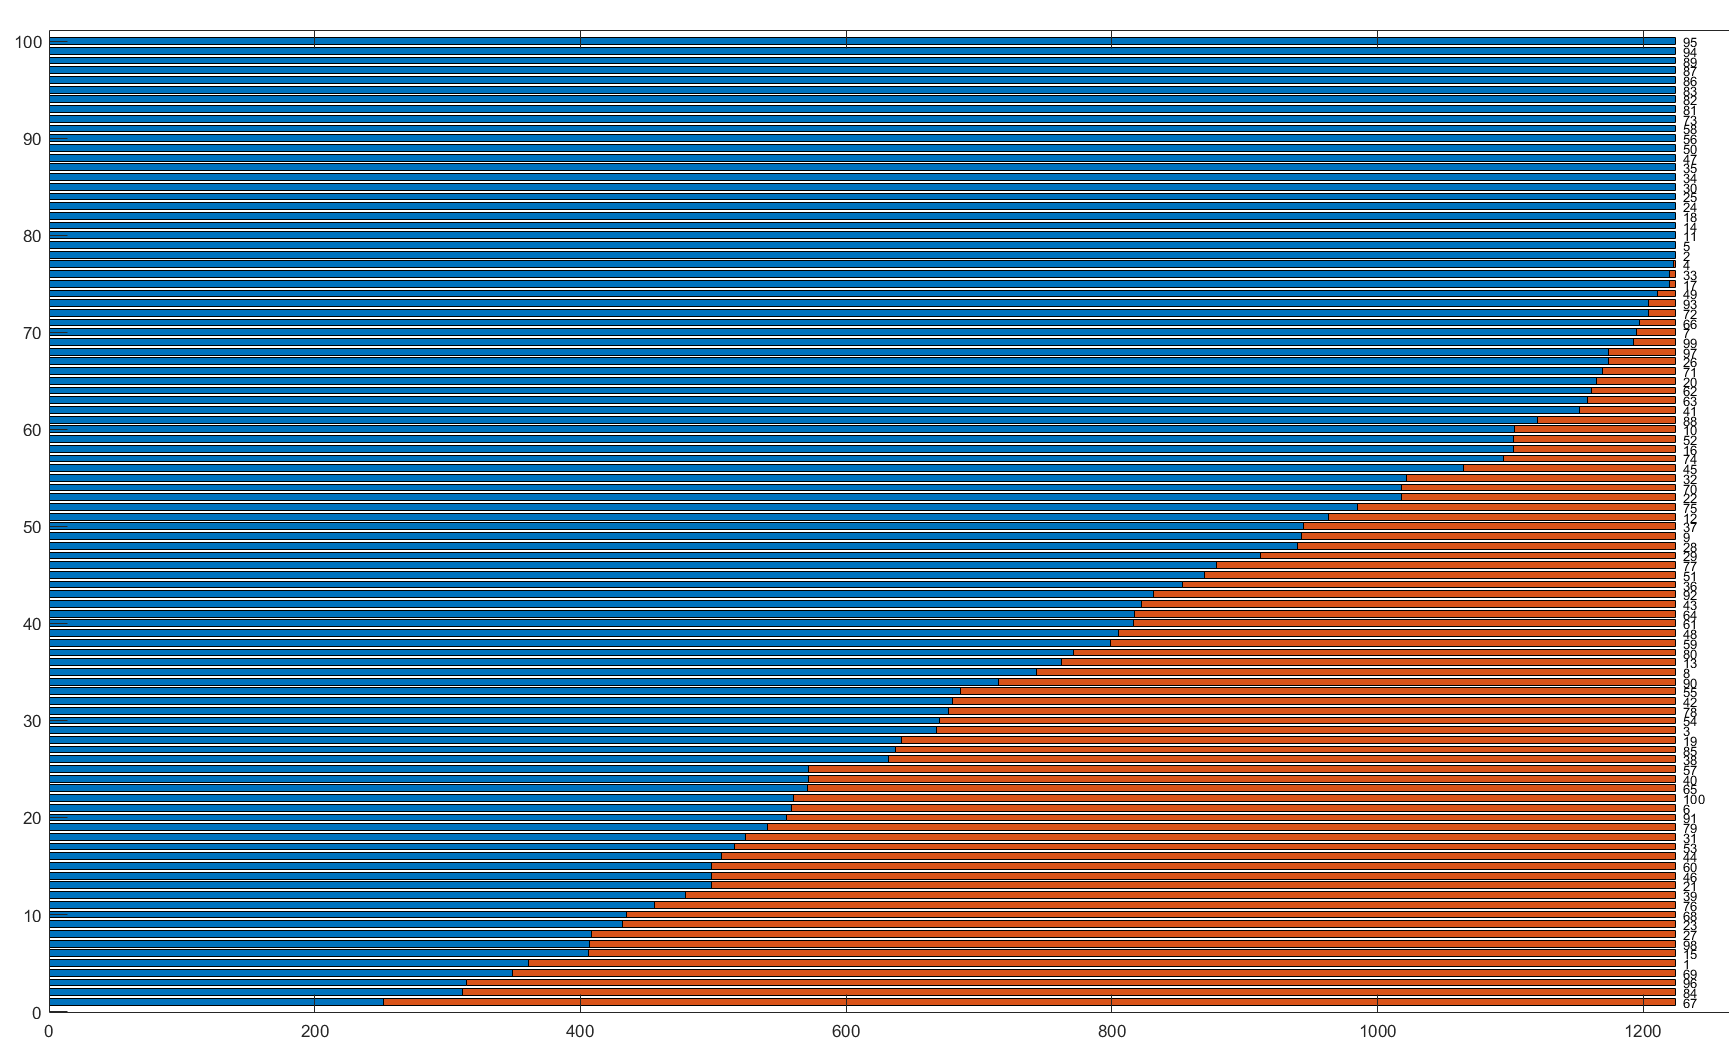
\includegraphics[scale=0.27]{imagenes/histo2_desafio6.png}
\caption{Ranking de exitos por clase para la prueba 2.}
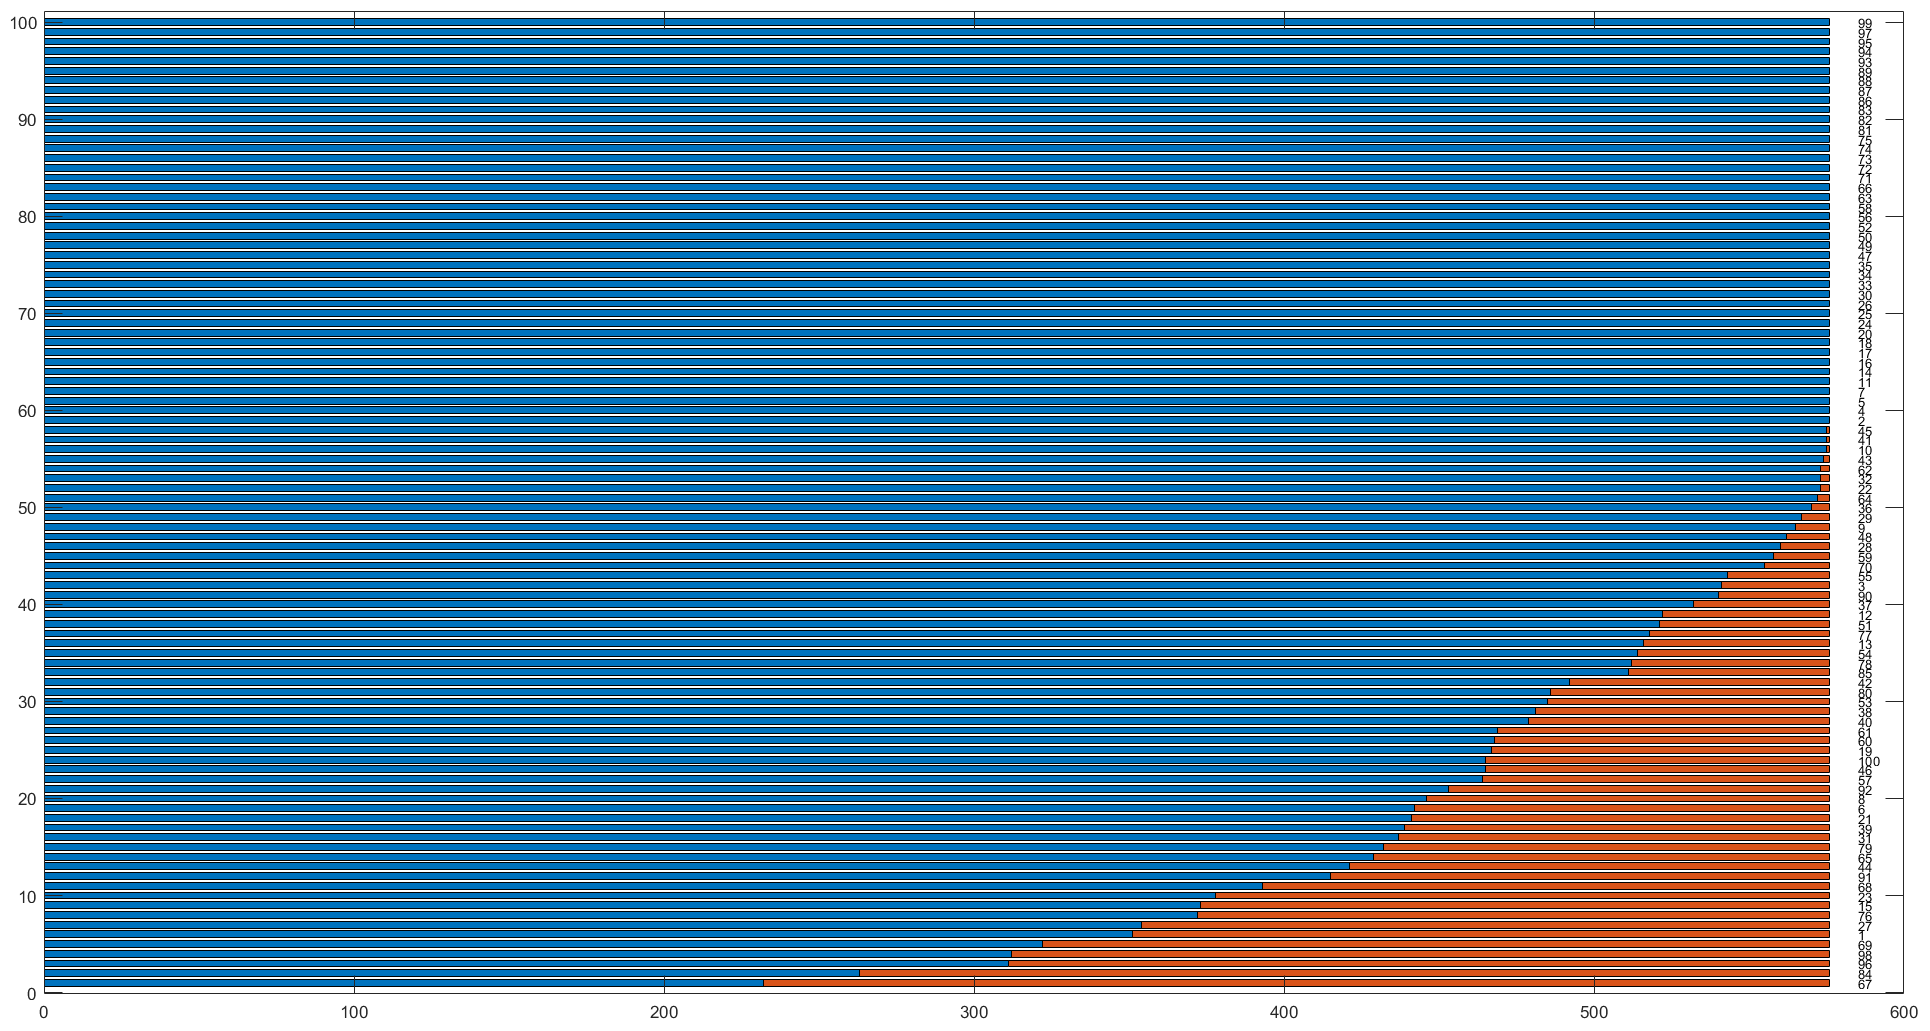
\includegraphics[scale=0.25]{imagenes/histo3_desafio6.png}
\caption{Ranking de exitos por clase para la prueba 3.}
\end{figure}


\pagebreak
\section{Desafío 7: Clasificar por características}

\subsection{Extracción de las características}
\paragraph{} En el siguiente desafío se utilizan varias herramientas de Matlab que sirven para extraer características de las imágenes, estas herramientas son \textit{detectSURFFeatures}, \textit{extractFeatures} y \textit{matchFeatures}. El siguiente código extraído de la documentación oficial de Matlab muestra un ejemplo de cómo utilizarlas.

\begin{lstlisting}

points1 = detectSURFFeatures(I1);
points2 = detectSURFFeatures(I2);

% Extract the features.
[f1,vpts1] = extractFeatures(I1,points1);
[f2,vpts2] = extractFeatures(I2,points2);

% Extract the features.
[f1,vpts1] = extractFeatures(I1,points1);
[f2,vpts2] = extractFeatures(I2,points2);

% Retrieve the locations of matched points.
indexPairs = matchFeatures(f1,f2) ;
matchedPoints1 = vpts1(indexPairs(:,1));
matchedPoints2 = vpts2(indexPairs(:,2));

% Display the matching points. The data still includes several outliers, but you can see the effects of rotation and scaling on the display of matched features.
figure; showMatchedFeatures(I1,I2,matchedPoints1,matchedPoints2);
legend('matched points 1','matched points 2');
\end{lstlisting}

\vspace*{1cm}
Si nos fijamos en la Figura 5 podemos ver como la mayoría de círculos rojos han coincidido con el objeto a buscar, el proceso que sigo para determinar la clase del objeto es buscar en la matriz de clases, que es una representación equivalente a la imagen de test pero con el valor de la clase en vez de los colores en cada posición como muestra la Figura 6, luego selecciono la clase con más ocurrencias.

\begin{figure}[hbtp]
\centering
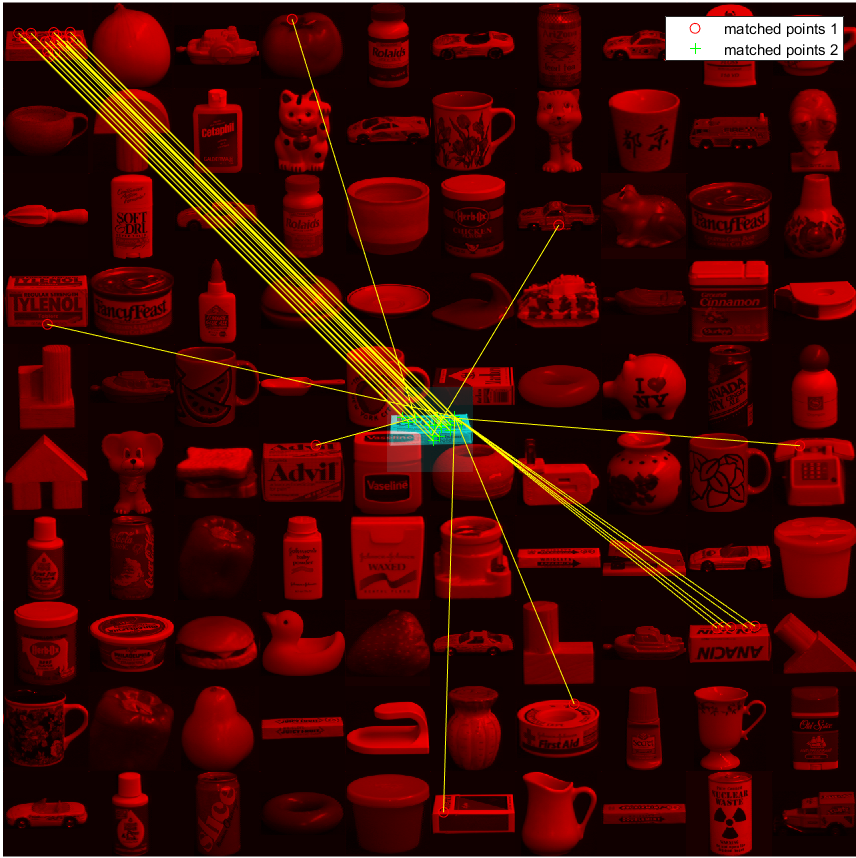
\includegraphics[scale=0.5]{imagenes/EscenaClasificacion.png}
\caption{Aplicación del código anterior una de las imágenes de coil-100.}


\includegraphics[scale=0.5]{imagenes/matrizClases.png}
\caption{Matriz de clases.}
\end{figure}

\pagebreak
\subsection{El conjunto de entrenamiento}
\paragraph{} Como conjunto de entrenamiento, utilizo una lista con las características de las imágenes de cada clase. La imagen de una clase puede ser bien una imagen individual o la unión de varias imágenes y esto viene definido por el parámetro \textit{ángulos}.\\ 

El siguiente código muestra como se crea la lista de características para cada clase y cómo se crean las imágenes en función de \textit{ángulos}.

\begin{lstlisting}
%% 
% Crea a partir de las imagenes  una lista de caracteristicas que luego se
% van a utilizar para encontrarlas en las escenas
%
function trainedFeatures = extractTrainFeatures(coil_100,angulos,h,w)
    trainedFeatures = cell(100,1);
    for i=1:100
        I = crearImagenDeEntrenamiento(coil_100, i, angulos,h,w);
       
        IG = rgb2gray(I);
        points = detectSURFFeatures(IG);
        [features,~] = extractFeatures(IG,points);
        trainedFeatures(i) = {features};
    end
end

%% Crea una union de imagenes 
%   
%
function I = crearImagenDeEntrenamiento(coil_100, clase, angulos,h,w)
    
    I=uint8(zeros(h*length(angulos),w,3));
    for i = 1:length(angulos)
        I((i-1)*h+1:i*h,1:w,1:3) = coil_100{clase,angulos(i)/5 + 1};
    end 
end

\end{lstlisting}
 \pagebreak
\subsection{El conjunto de test}
\paragraph{} En este desafío el conjunto de test está formado por una serie de escenas, una por cada ángulo donde cada escena es la unión de todas las imágenes de COIL-100 para ese ángulo.\\

La Figura 7 muestra la escena para el ángulo 0 y el siguiente fragmento de código contiene la función que crea tanto una escena como su matriz de clases (Figura 6).

\begin{lstlisting}
%% Crear Escena
% Une todas las imagenes de coil-100 para un angulo theta en una imagen de
% 10 x 10 imagenes.
%
% Crea una imagen equivalente donde cada coordenada tiene la clase
% perteneciente asociada.
%
% Muestra de imagenes 
function [muestra,matrizClases] = crearEscena(coil_100,theta,h,w)

    % Inicializamos la matriz que contendra todas las imagenes de muestra
    muestra=uint8(zeros(h*10,w*10,3));
    matrizClases = uint8(zeros(h*10,w*10));
    
    % Leemos las imagenes que tienen angulo Theta y creamos la escena con
    % ellas
    for i = 1:100
        
        % Calculamos los indices en los que se insertara la imagen
        [Q,R] = quorem(sym(i),sym(10));
        if R == 0
            R = 10;
            Q = Q - 1;
        end
        x = Q*h+1;
        x2 = (Q+1)*h;
        y = (R-1)*w + 1;
        y2 = R*w;
        
        % Anadimos la imagen a la escena y la clase a la matriz de clases
        muestra(x:x2,y:y2,1:3) = coil_100{i,theta};
        matrizClases(x:x2,y:y2) = i;
    end
end
\end{lstlisting}

\begin{figure}[hbtp]
\centering
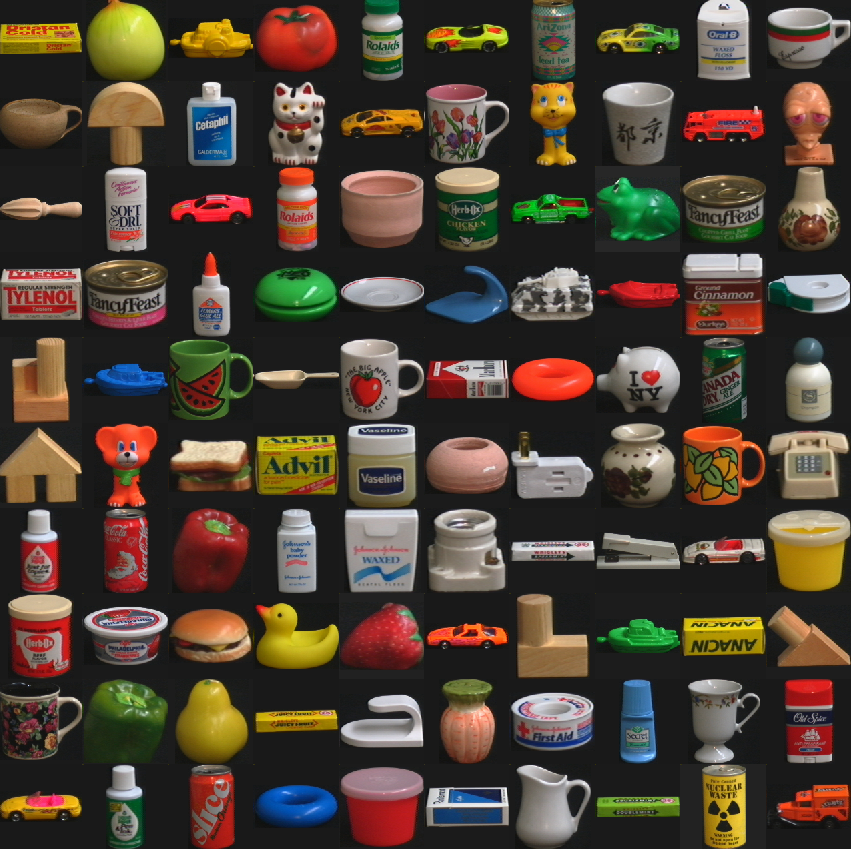
\includegraphics[scale=0.7]{imagenes/escena.png}
\caption{Escena con todas las imágenes de ángulo 0 de COIL-100.}
\end{figure}

\pagebreak
\subsection{Resultados}
\paragraph{} Utilizando el método explicado en la sección 5.1, he clasificado cada objeto en 72 escenas diferentes, y este proceso lo he repetido ampliando el número de representantes por objeto, la siguiente tabla muestra los resultados obtenidos.\\

\begin{tabular}{ccccc}
 \toprule
	\bfseries Prueba &
	\bfseries Ángulos de Rep.&
	\bfseries Escenas &
	\bfseries Media aciertos &
	\bfseries Est. Desv\\
 \midrule
	1 & 0 & 72 & 34.97 & 0.2256\\
	2 & 0, 90, 180, 270 & 72 & 54.63 &  0.2222\\
	3 & 0, 45, 90, 135, 180, 225, 270, 315 & 72 & 72.14 &  0.1629\\
 \bottomrule
\end{tabular}

\paragraph{}Los histogramas de las Figuras 8, 9 y 10, muestran el porcentaje de aciertos para cada escena, y pueden verse claramente como repuntan en las escenas que coinciden con los ángulos elegidos como representantes, ya que lógicamente habrá muchos más puntos en común entre estas imágenes.\\

La siguiente tabla muestra los objetos mejor y peor clasificados, en este caso es más complicado extraer conclusiones cue en los casos anteriores pero mi teoría es que 

\begin{tabular}{ccc|ccc}
 \toprule
	\bfseries Objeto &
    \bfseries \% Aciertos (p1) &
	\bfseries Imagen &
	\bfseries Objeto &
	\bfseries \% Aciertos (p3)&
	\bfseries Imagen\\
 \midrule
	50 & 100 & \adjustimage{height=2.8cm,valign=m}{imagenes/obj50__0} & 95 & 2.7 & \adjustimage{height=2.8cm,valign=m}{imagenes/obj95__0}\\
	\\
	33 & 98.6 & \adjustimage{height=2.8cm,valign=m}{imagenes/obj33__0} & 2 & 11.1 & \adjustimage{height=2.8cm,valign=m}{imagenes/obj2__0}  \\
	\\
	30 & 98.6 & \adjustimage{height=2.8cm,valign=m}{imagenes/obj30__0} & 70 & 19.4 & \adjustimage{height=2.8cm,valign=m}{imagenes/obj70__0}\\
	\\
	24 & 97.2 & \adjustimage{height=2.8cm,valign=m}{imagenes/obj24__0} & 75 & 19.4 & \adjustimage{height=2.8cm,valign=m}{imagenes/obj75__0} \\
 \midrule
 \bottomrule
\end{tabular}
    
\begin{figure}[hbtp]
\centering
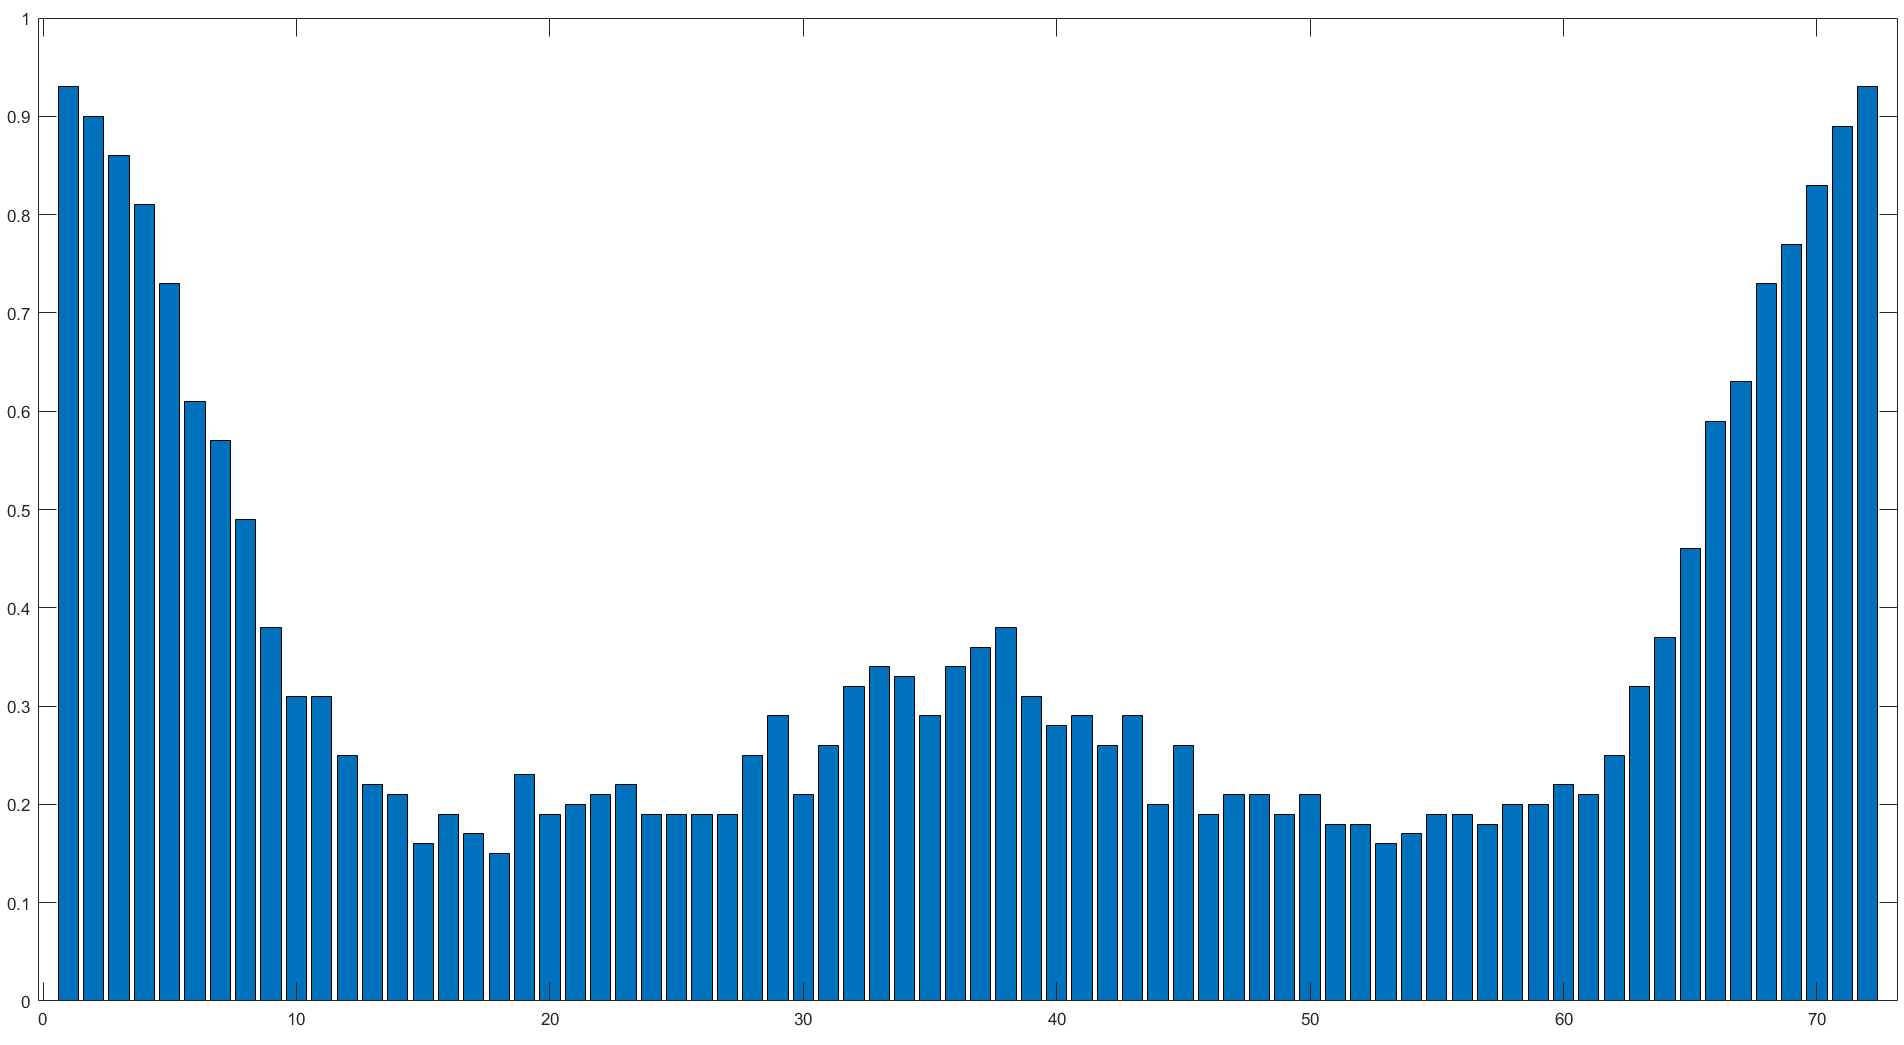
\includegraphics[width=0.7\linewidth]{imagenes/res72-0.png}
\caption{Porcentaje de aciertos por escena usando como representantes las imágenes de ángulo 0.}

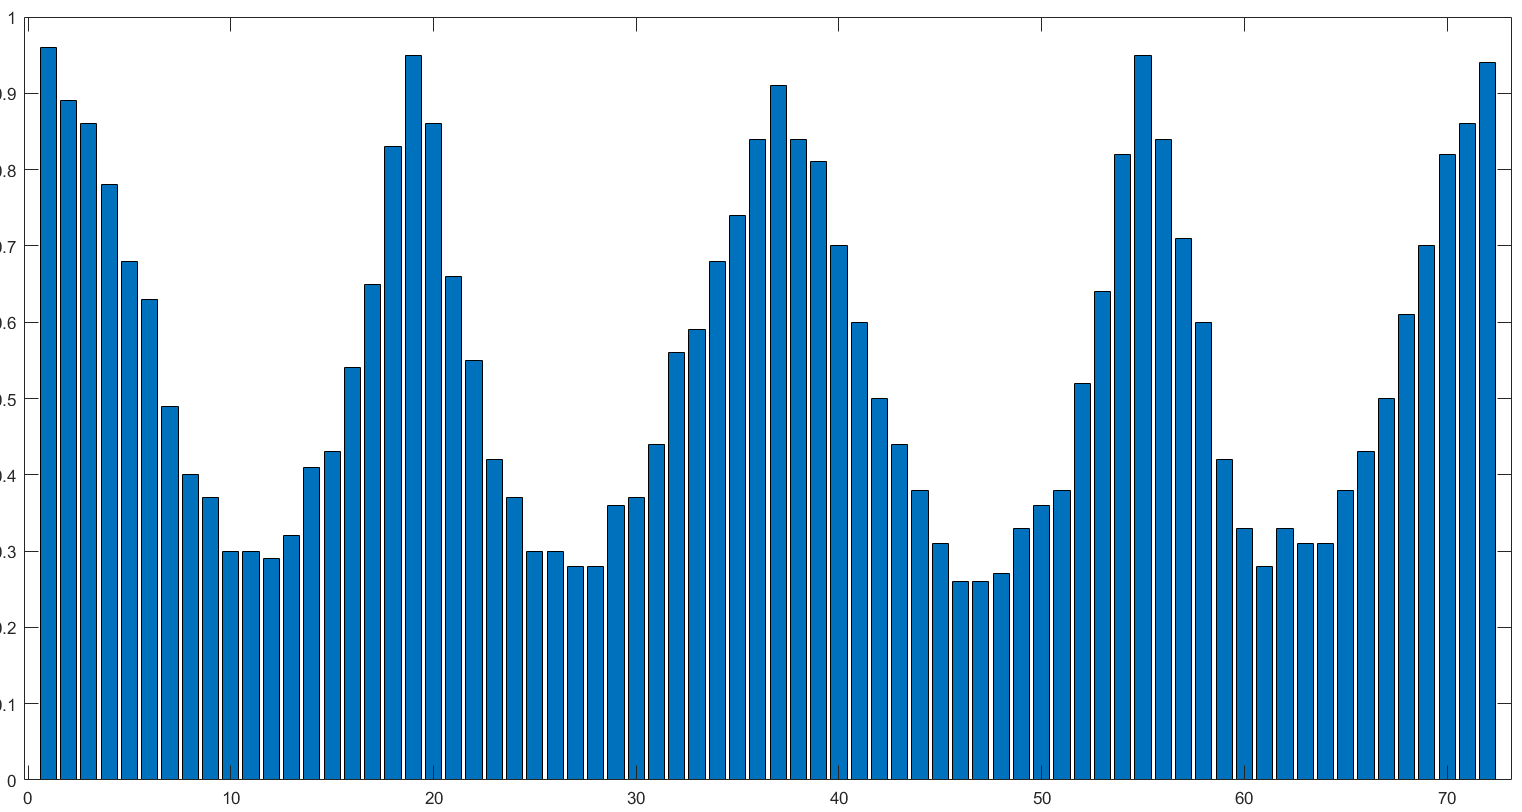
\includegraphics[width=0.7\linewidth]{imagenes/res72-4.png}
\centering
\caption{Porcentaje de aciertos por escena usando como representantes las imágenes de ángulo 0, 90, 180, 270.}

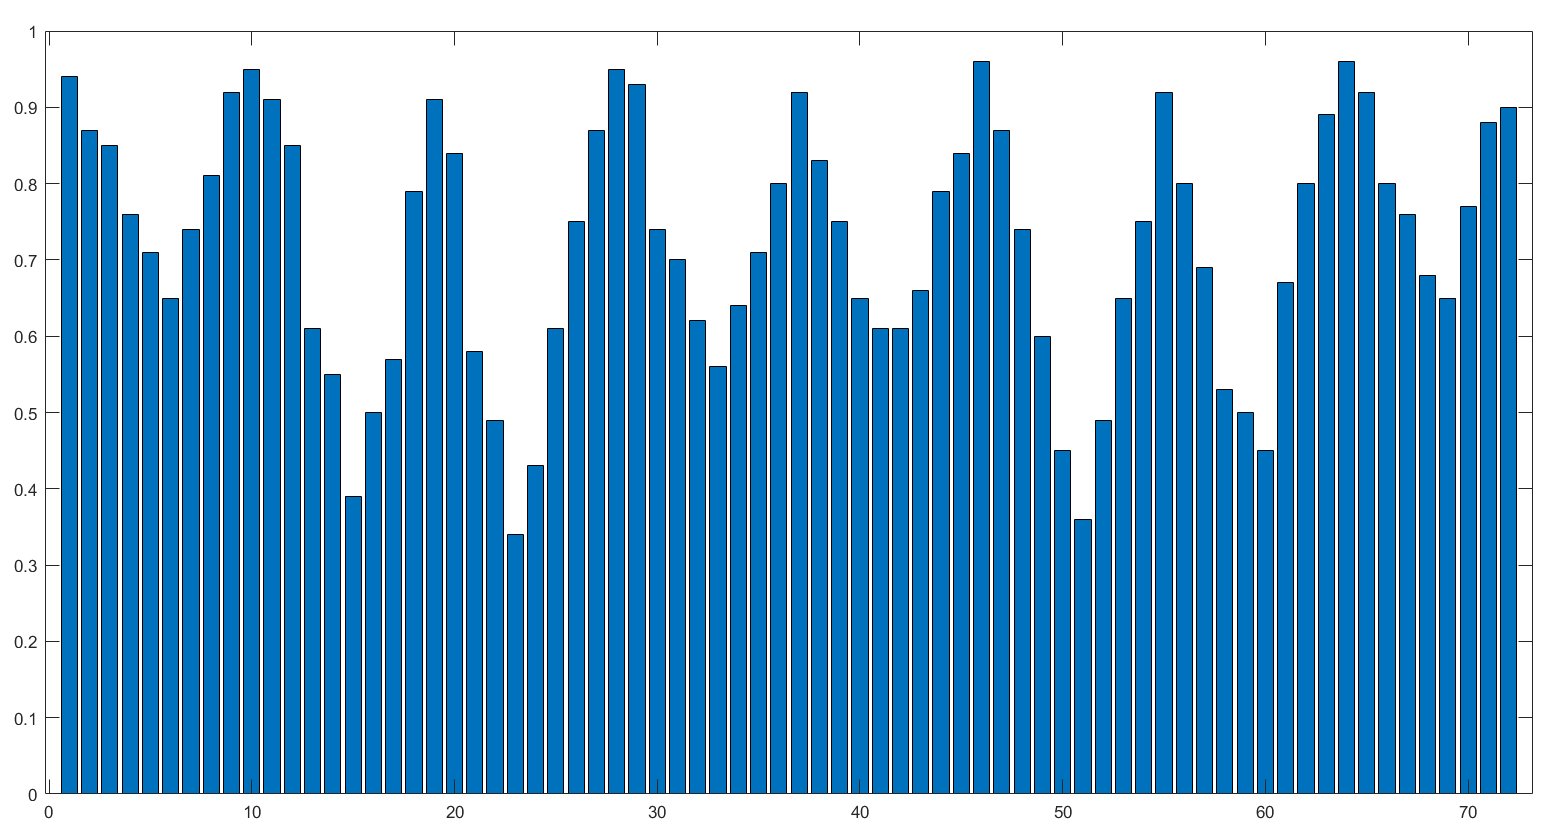
\includegraphics[width=0.7\linewidth]{imagenes/res72-8.png}
\centering
\caption{Porcentaje de aciertos por escena usando como representantes las imágenes de ángulo 0, 45, 90, 135, 180, 225, 270, 315.}\end{figure}

\begin{figure}[hbtp]
\centering
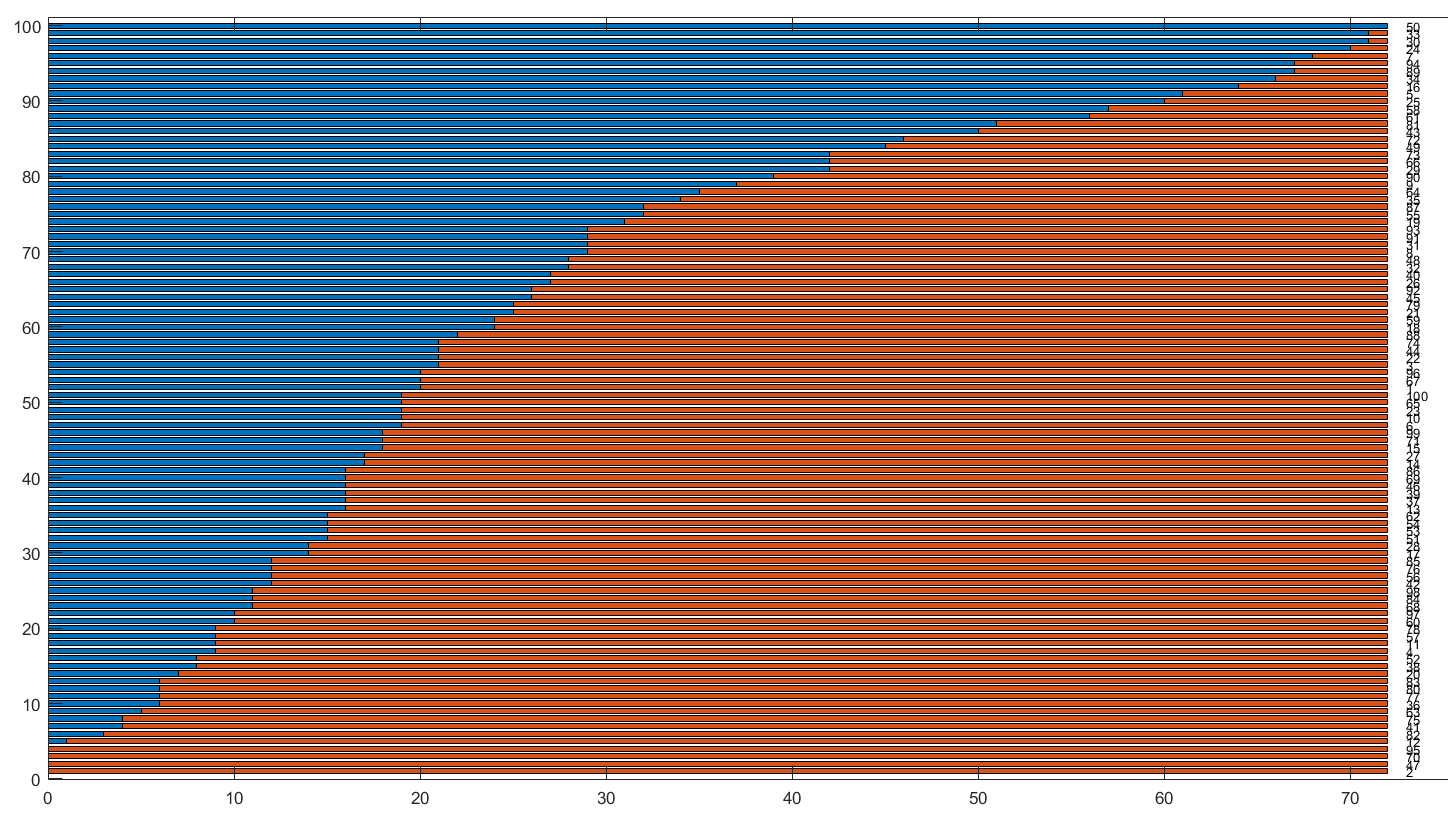
\includegraphics[scale=0.32]{imagenes/histo1_desafio7.png}
\caption{Ranking de exitos por clase para la prueba 1.}
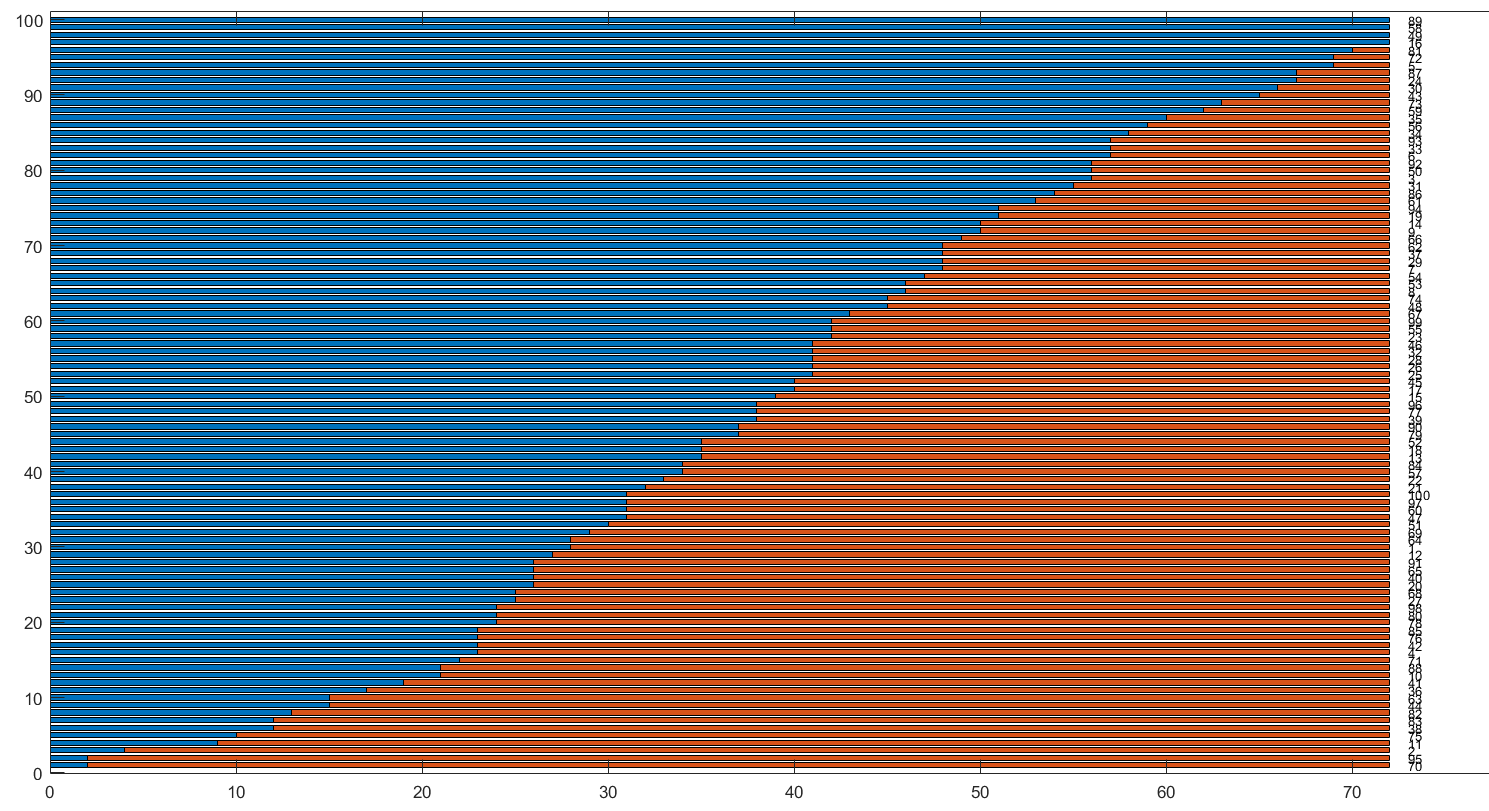
\includegraphics[scale=0.32]{imagenes/histo2_desafio7.png}
\caption{Ranking de exitos por clase para la prueba 2.}
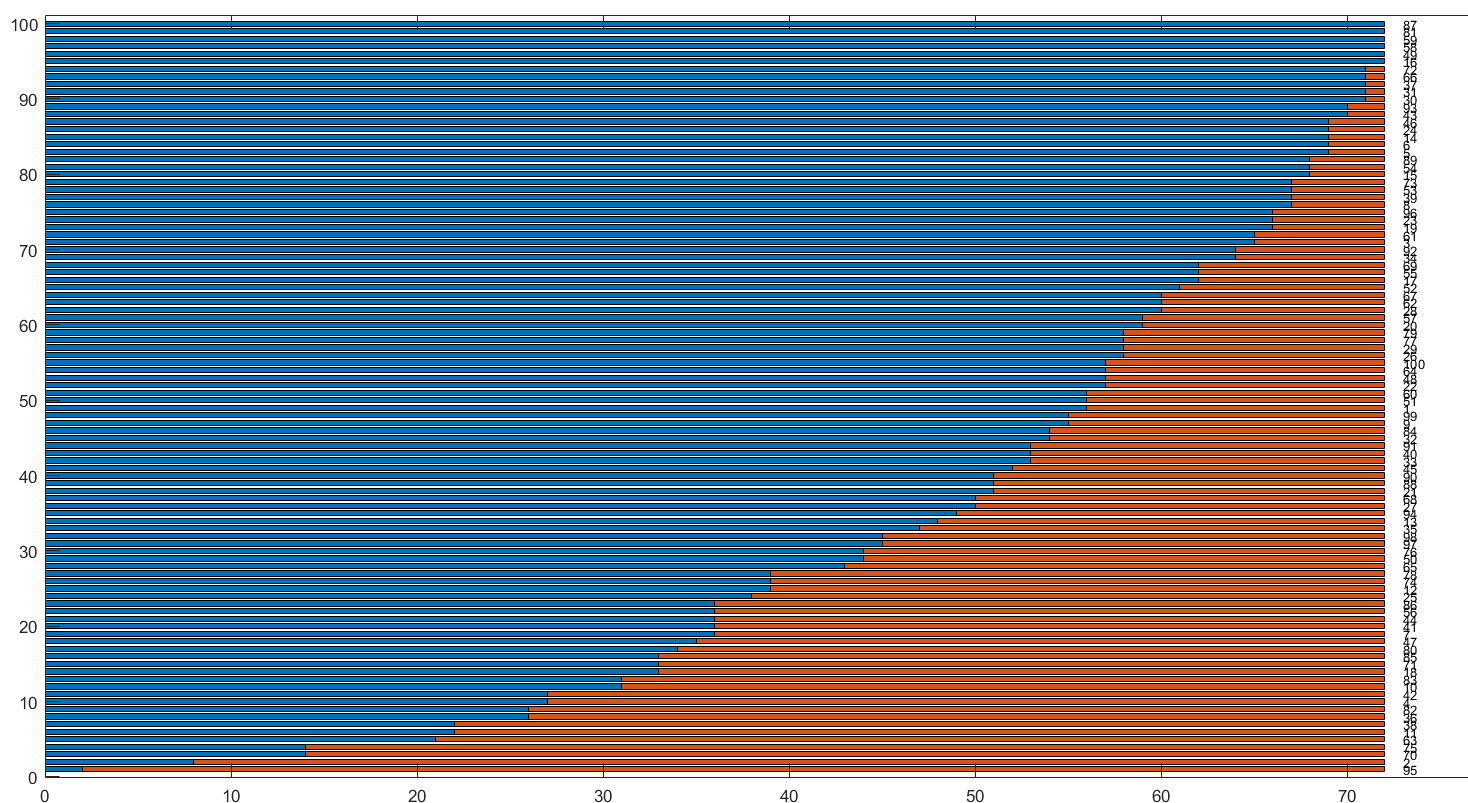
\includegraphics[scale=0.32]{imagenes/histo3_desafio7.png}
\caption{Ranking de exitos por clase para la prueba 3.}
\end{figure}

\pagebreak
\section{Anexos}
\subsection{Código completo desafío 5}
\begin{lstlisting}
%% Parametros de configuracion

clases = 100;         % Numero de clases
theta = 0 ;           % angulo de la imagen rotada de 0 a 355  (para el colormap)
colores = 256;        % Colores del indexado
h = 128;              % Alto de las imagenes
w = 128;              % Ancho de las imagenes
angulos = [0,90,180,270]; % Representantes

%% Main
[muestra,I,mct] = calcularMapaDeColores(clases,theta,h,w,colores);

reps = calcularRepresentantes(clases,angulos, mct);
clasificacion = clasificar(clases,reps,angulos,mct);
[confM,aciertos] = calcularResultados(clases,clasificacion);

%% Construir la muestra de colores
%%
%%
function [muestra,I,mct] = calcularMapaDeColores(clases,theta,h,w,colores)

    % Inicializamos la matriz que contendra todas las imagenes de muestra y de
    % la que extraeremos el mapa de colores con el que trabajar.
    %
    %  *Concatenaremos las imagenes en la primera dimension, por lo que los valores
    %   para la 2nda y la 3a dimension se mantienen iguales.
    %
    muestra=uint8(zeros(h*clases,w,3));

    % Leemos las imagenes que tienen angulo Theta y creamos el mapa de colores
    % con ellas
    for i = 1:clases

        % Rellenamos la muestra
        imageName = "obj"+i+"__"+theta+".png";
        muestra((i-1)*h+1:i*h,1:w,1:3) = imread(imageName);
    end
    
    % Extraccion del mapa de colores y muestra indexada a partir de la muestra
    [~,mct] = rgb2ind(muestra,colores);     
    I = rgb2ind(muestra,mct);     

end

% A partir de la muestra indexada, extraccion de cada histograma de colores que
% en este caso seran de tamano igual al mapa de colores (256)
% Matriz de celdas con los histogramas representantes de cada clase
function reps = calcularRepresentantes(clases,angulos, mct)
    reps = cell(clases*length(angulos),2);
    k = 1;
    % Para cada clase
    for i=1:clases
        % Para cada angulo en angulos de cada clase
        for j = 1:length(angulos)
            imageName = "obj"+i+"__"+angulos(j)+".png";
            [contadores,~]=imhist(rgb2ind(imread(imageName),mct),mct);
            reps(k,1:2)={i,contadores};
            k=k+1;
        end 
    end
end

%% Clasificacion de las imagenes
% En este punto todos los representantes estan creados y almacenados, ahora
% clasificamos el resto de las imagenes en funcion del valor de la norma
% para con cada representante, clasificando cada imagen como aquella con
% las menor distancia euclidea.
function clasificacion = clasificar(clases,reps,angulos,mct)

    % Matriz de pares con el numero de clase real y clasificado
    clasificacion = zeros(clases*(72 - length(angulos)),1);
    
    % Para cada clase de 1 a 100
    j = 1;
    for i = 1:clases
        % Para cada angulo de 0 a 355 (de 5 en 5 grados)
        for theta = 0:5:355
            if ~ismember(theta,angulos)
                imageName = "obj"+i+"__"+theta+".png";

                % Indexar y sacar el histograma
                indexada = rgb2ind(imread(imageName),mct);
                [contadores,~]=imhist(indexada,mct);

                % Clasificar
                clase = NN_1(reps,contadores);

                clasificacion(j,1:2) = [i, clase];
                j = j+1;
            end
        end 
    end
end

% NN_1 
%   
% reps -> lista de ( clase, histograma)
% aClasificar -> histograma
%
% returns clase de minima norma
%
function clase = NN_1(reps, aClasificar)
    
    min = intmax();
    clase = 0;
    
    for i = 1:length(reps)
        clase_temp = reps{i,1};
        hist = reps{i,2};
        norma = norm(hist-aClasificar);
        
        if norma < min 
            clase = clase_temp;
            min = norma;
        end 
    end
end

%% Extraccion de resultados de la clasificacion 
%
%
%
function [confM,aciertos] = calcularResultados(clases, clasificacion)
    confM = zeros(clases,clases);
    aciertos = 0;
    for i = 1:length(clasificacion)
        real = clasificacion(i,1); % Clase real
        clas = clasificacion(i,2); % Clase clasificada
        
        confM(real,clas) = confM(real,clas) + 1;
        
       if real == clas 
           aciertos = aciertos +1;
       end
    end
    
    aciertos = aciertos/length(clasificacion);
end
\end{lstlisting}
\pagebreak
\subsection{Código completo desafío 6}
\begin{lstlisting}

%% Leer los datos
caracteristicas = cell(100,72);
for obj=1:100
    for vista = 1:72
        imageName = "obj"+obj+"__"+(5*(vista-1))+".png";
        caracteristicas{obj,vista}=extractHOGFeatures(imread(imageName),'CellSize',[32, 32]);
    end
end

%%

confusion=zeros(100);

vistasTestSize = 8;
shift = 72/vistasTestSize;
for i=1:shift
    vistas_train = i:shift:i+(vistasTestSize-1)*shift;
    for vista_test=1:72
        if ~ismember(vista_test,vistas_train)
            for obj_test=1:100
                dist=[100*length(vistas_train) 2];
                
                k = 1;
                for obj_train=1:100
                    for j = 1:length(vistas_train)
                        dist(k,:)=[obj_train, norm(caracteristicas{obj_train,vistas_train(j)}-caracteristicas{obj_test,vista_test})];
                        k = k + 1;
                    end
                end

                [m,obj_m]=min(dist(:,2));
                obj_min = dist(obj_m,1);
                confusion(obj_test,obj_min)=confusion(obj_test,obj_min)+1;
            end
        end
    end
end

\end{lstlisting}
\pagebreak
\subsection{Código completo desafío 7}
\begin{lstlisting}
clases = 100;         % Numero de clases
h = 128;              % Alto de las imagenes
w = 128;              % Ancho de las imagenes
angulos = [0];        % Que imagenes van a usarse para el entrenamiento
 
% Cargar todas las imagenes para reducir operaciones I/O y tiempo de ejec.
coil_100 = loadCoilDatabase();
 
% Extraer las caracteristicas de las imagenes 
trainedFeatures = extractTrainFeatures(coil_100,angulos,h,w);

for j = 1:72
    % Creo la escena de imagenes y la de sus clases correspondientes
    [escena,matrizClases] = crearEscena(coil_100,j, h, w);

    % Extraer las caracteristicas SURF (Speeded-Up Robust Features algorithm)
    % de la escena
    escenaGS = rgb2gray(escena);
    pointsEscena = detectSURFFeatures(escenaGS);
    [featuresEscena,validPointsEscena] = extractFeatures(escenaGS,pointsEscena);

    % Busco cada imagen en la escena usando las caracteristicas entrenadas
    % al principio
    clasificacion = zeros(100,2);
    for i = 1:100
        clasificacion(i,:) = [i,clasificarImagen(trainedFeatures{i}, featuresEscena, validPointsEscena, matrizClases)];
    end
    
    resultados(j) =  calcularAciertos(clasificacion);
end

%% 
% Crea a partir de las imagenes  una lista de caracteristicas que luego se
% van a utilizar para encontrarlas en las escenas
%
function trainedFeatures = extractTrainFeatures(coil_100,angulos,h,w)
    trainedFeatures = cell(100,1);
    for i=1:100
        I = crearImagenDeEntrenamiento(coil_100, i, angulos,h,w);
       
        IG = rgb2gray(I);
        points = detectSURFFeatures(IG);
        [features,~] = extractFeatures(IG,points);
        trainedFeatures(i) = {features};
    end
end


%% Clasificar imagenes
%%
function clase = clasificarImagen(features, featuresEscena, validPointsEscena, matrizClases)
    
    % Buscar coincidencias entre las caracteristicas
    indexPairs = matchFeatures(featuresEscena,features) ;

    % Extraer puntos de la escena que han coincididio
    matchedPointsEscena = validPointsEscena(indexPairs(:,1));
    
    % Buscar en la matriz de clases los puntos que han coincidido y extraer
    % las clases
    clases = zeros([matchedPointsEscena.Count 1]);
    locations = matchedPointsEscena.Location;
    for i = 1:matchedPointsEscena.Count
        clases(i) = matrizClases(floor(locations(i,2)),floor(locations(i,1)));
    end     
    
    % Elegir la clase mas frecuente como la clasificada
    clase = mode(clases);
   
    if isnan(clase)
        clase = 1;
    end
end

%% Crear Escena
% Une todas las imagenes de coil-100 para un angulo theta en una imagen de
% 10 x 10 imagenes.
%
% Crea una imagen equivalente donde cada coordenada tiene la clase
% perteneciente asociada.
%
% Muestra de imagenes 
function [muestra,matrizClases] = crearEscena(coil_100,theta,h,w)

    % Inicializamos la matriz que contendra todas las imagenes de muestra
    muestra=uint8(zeros(h*10,w*10,3));
    matrizClases = uint8(zeros(h*10,w*10));
    
    % Leemos las imagenes que tienen angulo Theta y creamos la escena con
    % ellas
    for i = 1:100
        
        % Calculamos los indices en los que se insertara la imagen
        [Q,R] = quorem(sym(i),sym(10));
        if R == 0
            R = 10;
            Q = Q - 1;
        end
        x = Q*h+1;
        x2 = (Q+1)*h;
        y = (R-1)*w + 1;
        y2 = R*w;
        
        % Anadimos la imagen a la escena y la clase a la matriz de clases
        muestra(x:x2,y:y2,1:3) = coil_100{i,theta};
        matrizClases(x:x2,y:y2) = i;
    end
end

%% Extraccion de resultados de la clasificacion 
%
%
%
function aciertos = calcularAciertos(clasificacion)
    %confM = zeros(clases,clases);
    aciertos = 0;
    for i = 1:length(clasificacion)
        real = clasificacion(i,1); % Clase real
        clas = clasificacion(i,2); % Clase clasificada
%         if clas ~= 0
%             confM(real,clas) = confM(real,clas) + 1;
%         end
       if real == clas 
           aciertos = aciertos +1;
       end
    end
    
    aciertos = aciertos/length(clasificacion);
end

%% Crea una union de imagenes 
%   
%
function I = crearImagenDeEntrenamiento(coil_100, clase, angulos,h,w)
    
    I=uint8(zeros(h*length(angulos),w,3));
    for i = 1:length(angulos)
        I((i-1)*h+1:i*h,1:w,1:3) = coil_100{clase,angulos(i)/5 + 1};
    end 
end

%% Carga todas las imagenes de coil
function coil_100 = loadCoilDatabase()
    coil_100 = cell(100,72); 
    for i = 1:100
        for j = 0:5:355
            coil_100(i,j/5+1) = {imread("obj"+i+"__"+j+".png")};
        end
    end
end
\end{lstlisting}
\begin{thebibliography}{arauak}
	
	\bibitem[1]{key-1} Matlab documentación oficial:\textit{es.mathworks.com}
	
	\bibitem[2]{key-2} COIL-100, http://www.cs.columbia.edu/CAVE/software/softlib/coil-100.php
	
\end{thebibliography}



\end{document}
